The purpose is to predict the total hourly wind production available on the energy market from all of western Denmark (DK1) with enough accuracy to make a green decision. It is important to note that it is the wind production available on the market and not the entire production of Western Denmark. The entire wind production would be much higher and is not all distributed through the deregulated market\ref{FIND ONE} - fx. vindstoed and private owned. This can also be seen by the correlation between consumption and wind production in Table~\ref{table:pearsonCoeficientWindProduction} and Figure~\ref{fig:consumptionVsWindProduction} which indicates that the production is moved into the market when the demand for electricity is high. Because the wind production follows market trends it is necessary to consider economical and statistical factors of the current market situation when predicting the production. It is our intention to get a close enough estimate so that it can be used as an indicator for the hourly amount of wind production in the market for the next 24 hours.
Most others have been forecasting the wind production for specific wind farms where exact weather conditions and wind mill throughput of the site was known. We do not. This is also more critical in the other examples because it is used to place the mills or the predict how much electricity the mill can sell the next year - a large investment would be lost if placed wrong. 

It is not surprising that weather conditions directly impact the wind power generation. The typical input parameters for wind power prediction are wind speed, air density, temperature and pressure \cite{WindPowerGenerationUsingANN} with the most influential factor being wind speed because it is directly converted to power in the wind turbine. The following subsections will describe the parameters relationship to wind production and how it is used in the modelled ANN.

The Pearson Correlation Coefficient\footnote{\url{http://en.wikipedia.org/wiki/Pearson_product-moment_correlation_coefficient}} has been used to establish the linear dependency between meteorological factors, consumption and wind production. Table ~\ref{table:pearsonCoeficientWindProduction} shows this correlation coefficient. The factors have been discussed throughout the thesis as having an influence on the wind speed production to some degree. The Pearson Correlation Coefficient returns a value between -1 and +1 which indicates the strength of the linear correlation between two variables.

\begin{table}[H]
\centering  % used for centering table
\begin{tabular}{c c} % centered columns (3 columns)
Input factor & Pearson Correlation Coefficient \\ [0.5ex] % inserts table 
%heading
\hline                  % inserts single horizontal line
Consumption & 0.62 \\ % inserting body of the table
Wind Speed & 0.94 \\
Temperature & -0.09 \\
Wind Direction & 0.21 \\ [1ex] % [1ex] adds vertical space
\hline %inserts single line
\end{tabular}
\caption{Table showing Pearson correlation coefficient between various factors and the wind production.} % title of Table
\label{table:pearsonCoeficientWindProduction} % is used to refer this table in the text
\end{table}

It is obvious from Table~\ref{table:pearsonCoeficientWindProduction} that consumption and wind speed are the most direct influential factors. The consumption or demand can become a problem because it also needs to be predicted and if this prediction shows to be inaccurate then it will add the error to the wind production forecast.  (ADD MORE LIKE DENSITY, DEW POINT, HUMIDITY, TIME OF DAY, ECT).

\subsection{Wind Speed}
The relationship between hourly wind speed and hourly wind power production of DK1 is seen in Figure~\ref{fig:windVsProd}. The graph clearly shows the expected impact of wind speed on the wind energy production.

\begin{figure}[H]
\centering
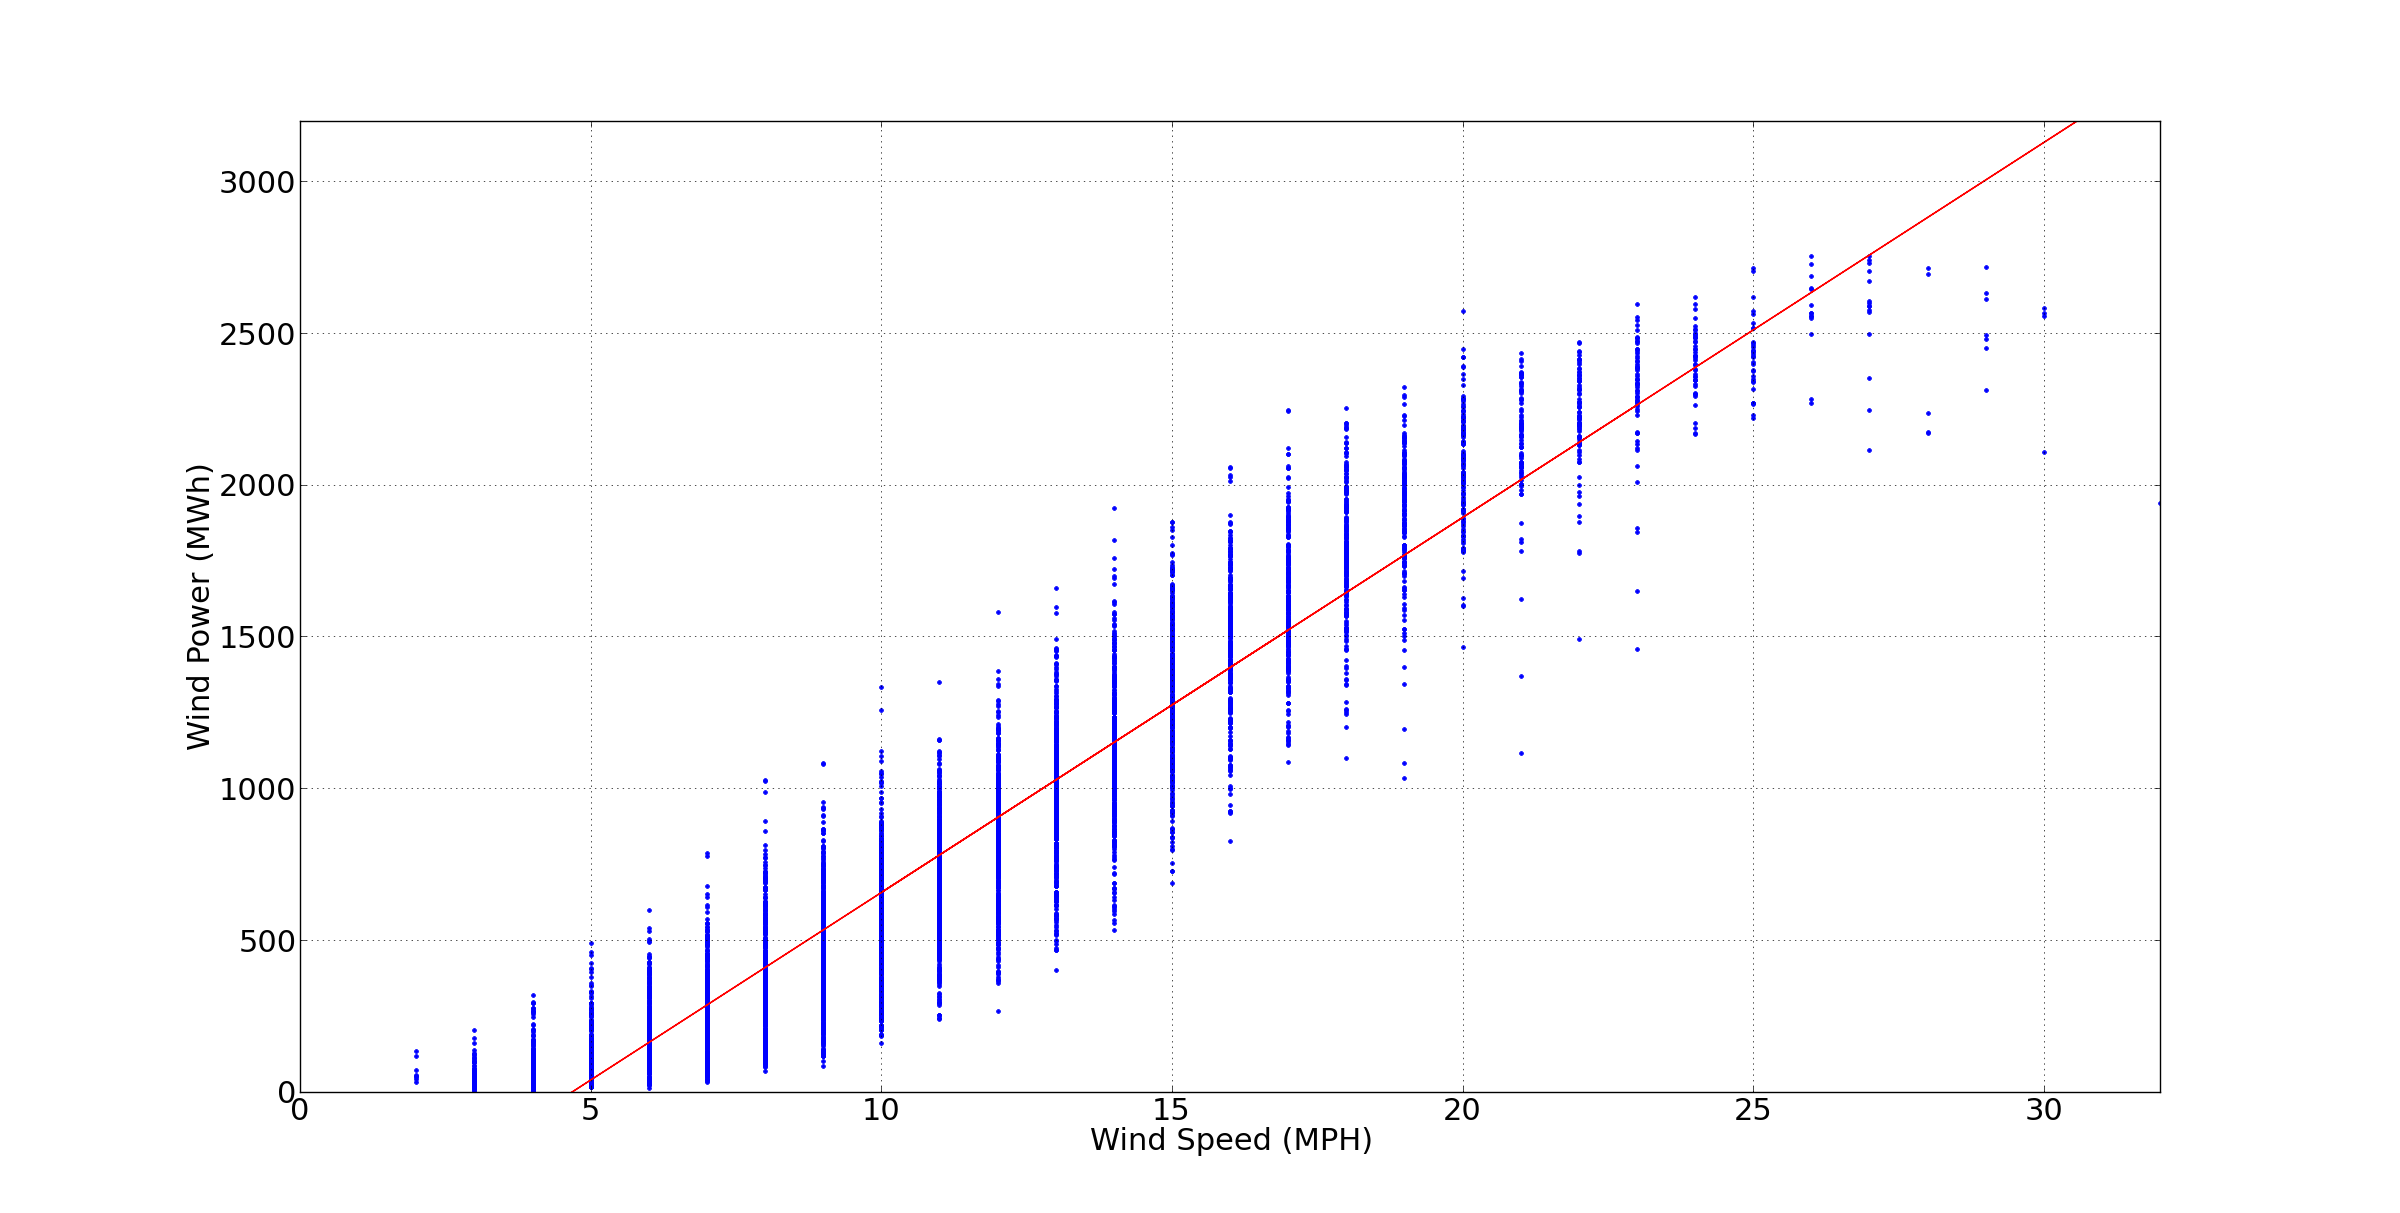
\includegraphics[width=0.99\linewidth,natwidth=898,natheight=587]{billeder/WindSpeedVsProduction.png}
\caption{Wind speed vs. wind production in 2012}
\label{fig:windVsProd}
\end{figure}

What is noticeable from the graph is wide range of productions that is covered by a relatively small number of wind speeds. Wind speed 15 can cover wind productions all the way from 700 to 1900 and therefore other input parameters are needed to point us in the right direction within these interval. 

\subsection{Air Density}
It is described in ~\ref{sec:windmillPlacement} that wind energy is proportional to air density where a higher density means more power for a specific wind speed. This does not imply that a higher air density is equal to higher wind power production in general because it depends on the wind speed. Days with equal wind speed but variation in air density should show an increase in power production when the air density is highest. 

Air density depends directly on temperature and pressure which can be described by $Air Density=\frac{P*M}{(R*T)}$ where R is a gas constant and M is the density of air. The monthly pressure in Denmark has low variation compared to the temperature as shown in Figure~\ref{fig:pressureTemperatureVariance}. For this reason, the temperature will have the most influence on the air density in Denmark. The formula express that when temperature decreases the air density will increase linearly, e.g. the wind power production for a specific wind speed will be higher in times of low temperature. The air density has been calculated for every hour in the training set and the correlation has been established for each wind speed in Table~\ref{table:pearsonCoeficientAirDensity}. The wind power production increases with the air density for each wind speed as described by the formula.

\begin{figure}[H]
\centering
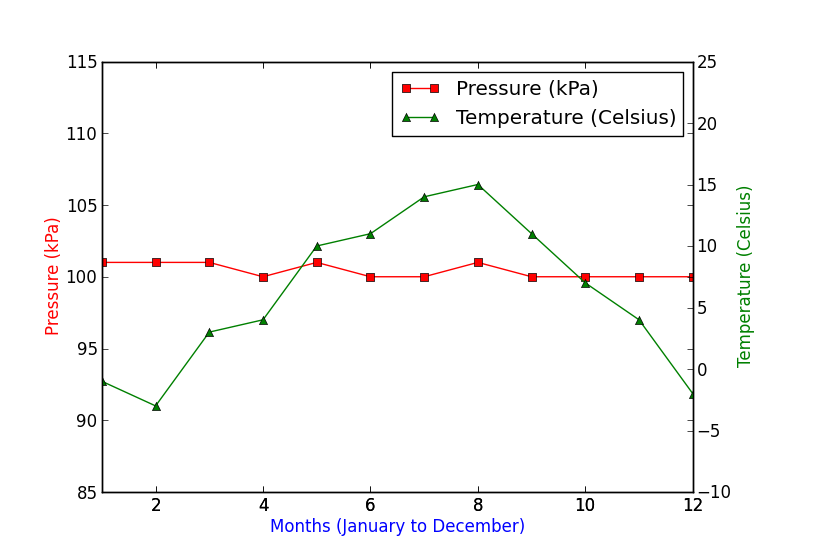
\includegraphics[width=0.99\linewidth,natwidth=898,natheight=587]{billeder/pressureTemperatureVariance.png}
\caption{Temperature and Pressure variance for 2012}
\label{fig:pressureTemperatureVariance}
\end{figure}

\begin{table}[H]
\centering  % used for centering table
\begin{tabular}{c c} % centered columns (3 columns)
Wind Speed (mph) & Pearson Correlation Coefficient for Air Density \\ [0.5ex] % inserts table 
%heading
\hline                  % inserts single horizontal line
2 & 0.299137300509 \\ \hline
3 & 0.3796284049 \\ \hline
4 & 0.282639503931 \\ \hline
5 & 0.176882800847 \\ \hline
6 & 0.26624422678 \\ \hline
7 & 0.257509841245 \\ \hline
8 & 0.293342212093 \\ \hline
9 & 0.306523814111 \\ \hline
10 & 0.279322572227  \\ \hline
11 & 0.18103337532 \\ \hline
12 & 0.187564572882 \\ \hline
13 & 0.18967147434 \\ \hline
14 & 0.186865264412 \\ \hline
15 & 0.11895069643 \\ \hline
16 & 0.0935379251673 \\ \hline
17 & 0.218516563436 \\ \hline
18 & 0.113577325408 \\ \hline
19 & 0.280301272164 \\ \hline
20 & 0.0938772997337 \\ \hline
21 & 0.180318818497 \\ \hline
22 & 0.176361903194 \\ \hline
23 & 0.259569218995 \\ \hline
24 & 0.012949223523 \\ \hline
25 & 0.116039820562 \\ \hline
26 & 0.197093832088 \\ \hline
27 & 0.71694505409 \\ \hline
28 & 0.867450709217 \\ \hline
29 & 0.61036610708 \\ \hline
30 & 0.758217075936 \\ \hline  
Average: & 0.279325455487 \\ [1ex] % [1ex] adds vertical space      
\hline %inserts single line
\end{tabular}
\caption{Table showing Pearson correlation coefficient between the various wind speeds in the dataset and the air density.} % title of Table
\label{table:pearsonCoeficientAirDensity} % is used to refer this table in the text
\end{table}

\subsection{Wind Direction}
bla bla intro. Figure~\ref{fig:windDirVsProd} shows that western wind has a tendency to produce more energy. (need to further investigated but seems valid when looking at dk).
\begin{figure}[H]
\centering
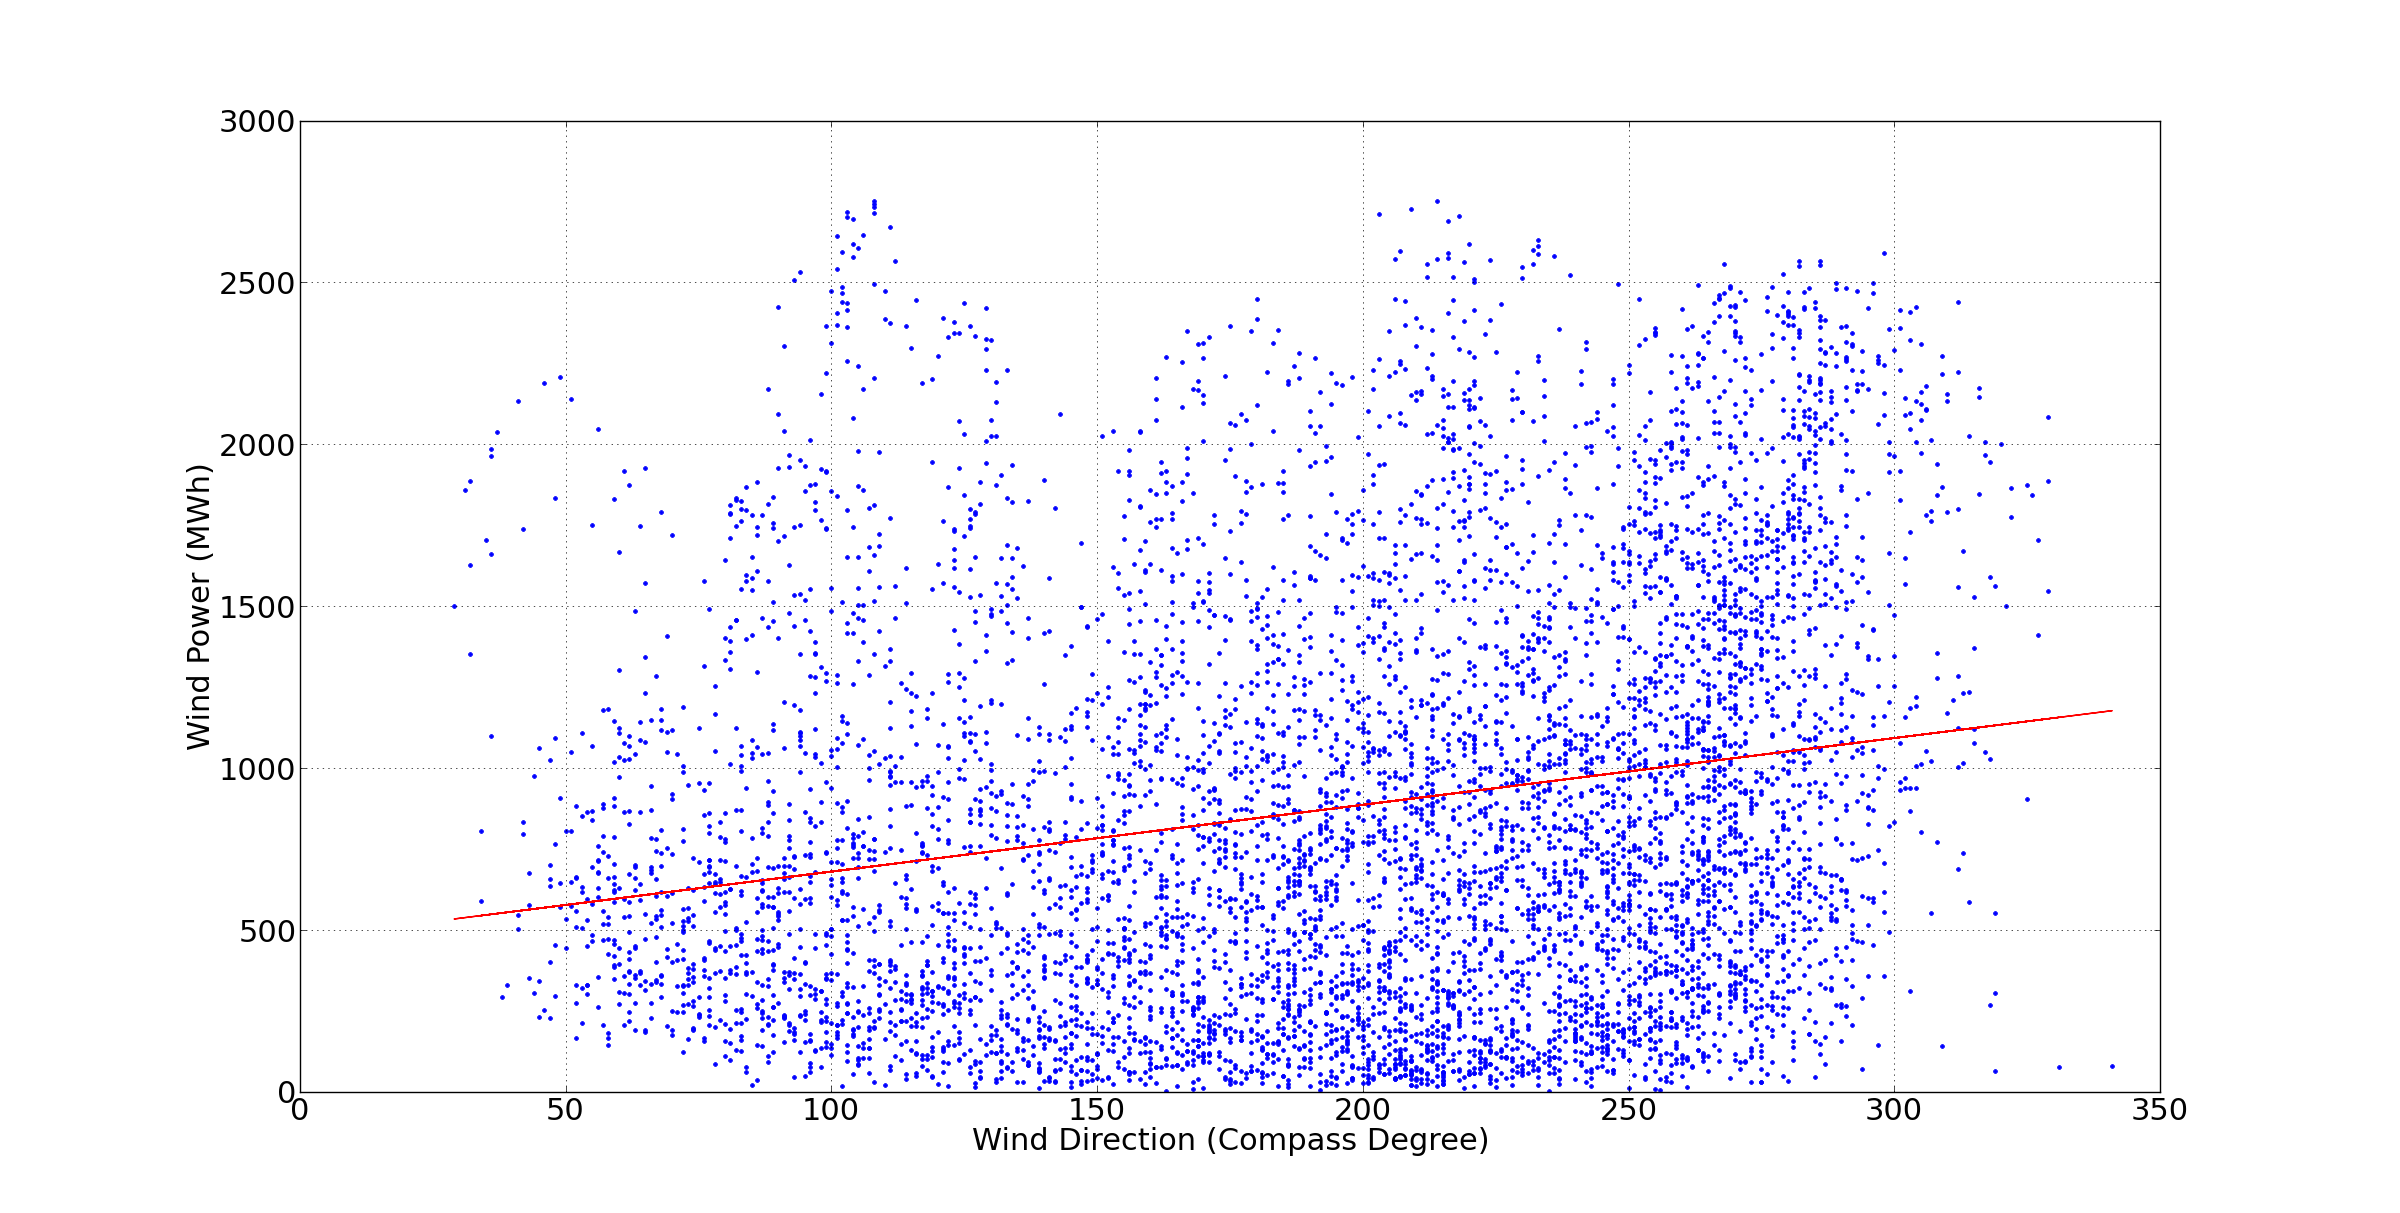
\includegraphics[width=0.99\linewidth,natwidth=898,natheight=587]{billeder/productionVsWindDirection.png}
\caption{Wind Direction vs. wind production in 2012}
\label{fig:windDirVsProd}
\end{figure}

\subsection{Consumption}
It is expected that the wind power available on the energy market will be low at times with low consumption, e.g if no energy is needed the wind power can't be sold.  This relationship is shown in Figure~\ref{fig:consumptionVsWindProduction}. This also tells us that the wind production is connected to the market and cannot be deduced only from meteorological factors.

\begin{figure}[H]
\centering
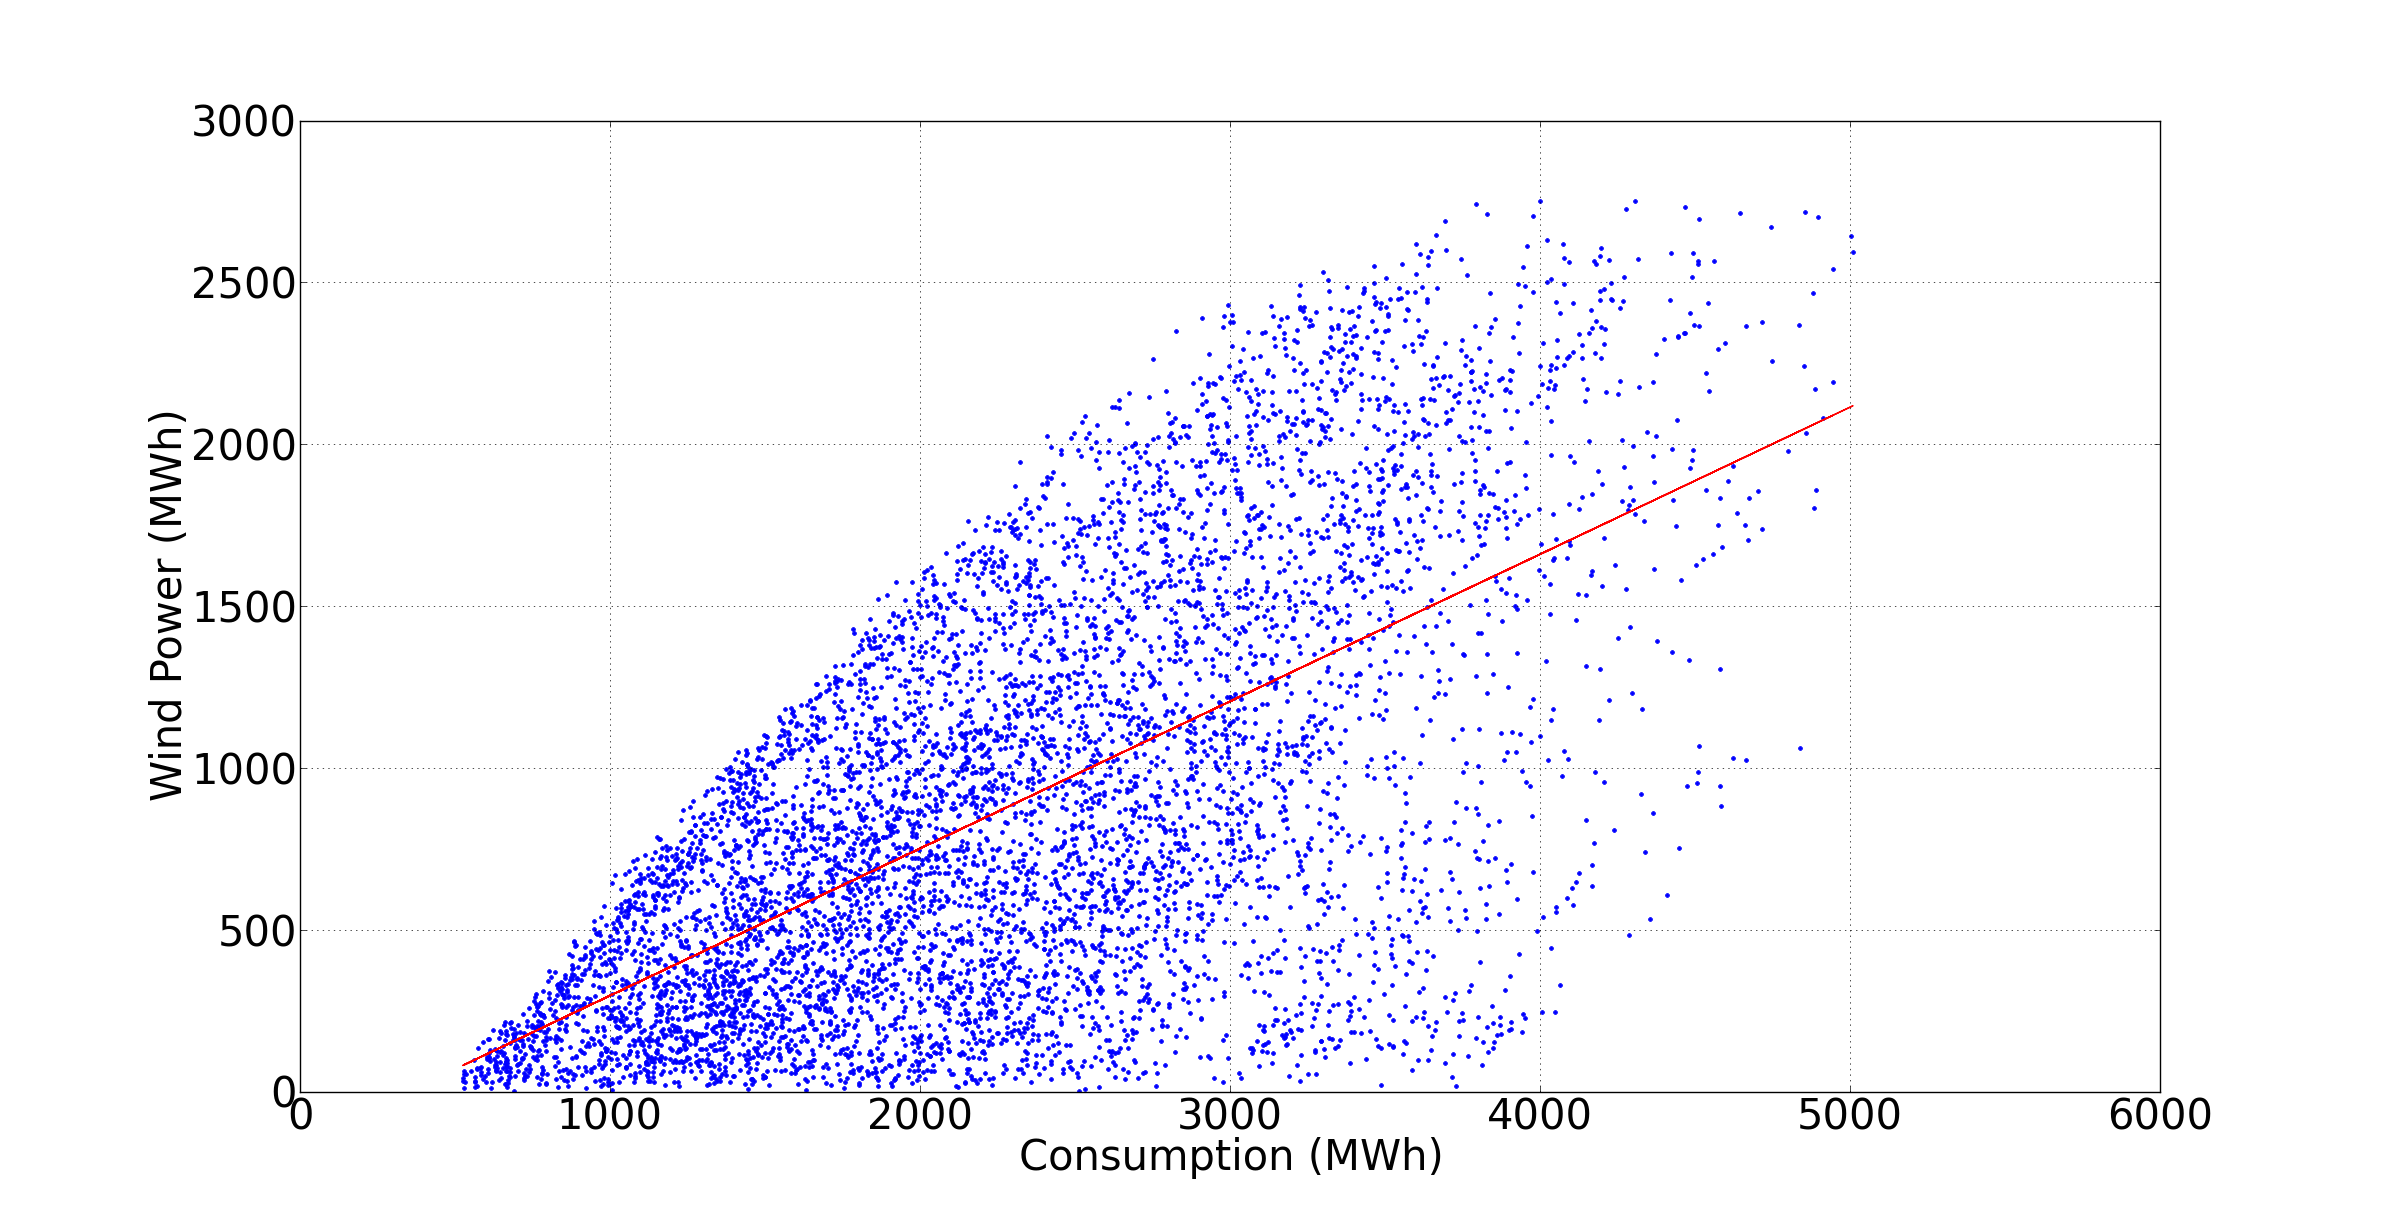
\includegraphics[width=0.99\linewidth,natwidth=898,natheight=587]{billeder/consumptionVsWindProduction.png}
\caption{Consumption vs. Wind Production in 2012}
\label{fig:consumptionVsWindProduction}
\end{figure}

\subsection{Time of day}
The dataset consists of all hours of the years included. Based on this the network is going to forecast multiple hours ahead and it therefore necessary to establish if any correlation between the time of day and the wind production exist. The average wind production distribution for a calendar day can be seen in Figure~\ref{fig:hourly_wind_production}. The wind production is at its highest during the day from 8-20 and therefore it is needed to use the time of day as input parameters.  

\begin{figure}[H]
\centering
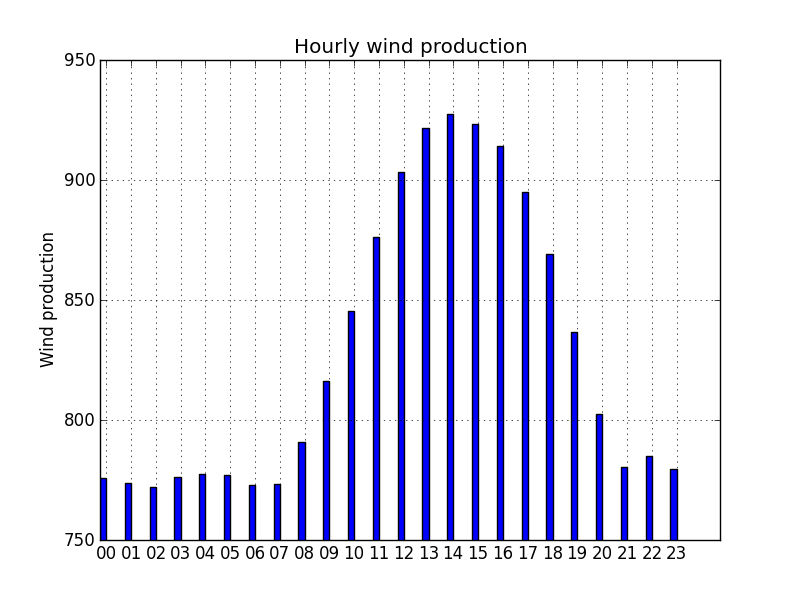
\includegraphics[width=0.99\linewidth,natwidth=898,natheight=587]{billeder/hourly_wind_production.png}
\caption{Time of day vs. Wind Production in 2012}
\label{fig:hourly_wind_production}
\end{figure}

\subsection{Wind Production Development}
The above analysis shows the wind production development to be much dependent on wind speed and air density together with the general trend on the market. The need for identifying trends is discussed here~\ref{sec:usingStatisticalInput}. 

The high volatility in the wind production is very clear when considering the development curve in Figure~\ref{fig:windHourDevelopment400Hours}. This is not a problem if the correlation between the input parameters result in a low number of output possibilities because the generalization of the ANN then would be enough. This is not the case for our input parameters for wind productions and an example of such can be seen in ~\ref{fig:inputParameterDistribution} where outputs for similar inputs are shown --- the input limits can be seen in Table~\ref{table:similarHoursLimitsWindProd}. The generalization would lean towards 898-1048 but if the last wind production was 1198 and the tendency rising then the prediction would be better off guessing above or around 1198. This can be further supported by Figure~\ref{fig:windHourDevelopment400Hours} which illustrates the tendency of the production curve and the need to consider the immediate past because of its significance for the movements to come. It is necessary to identify these tendencies in every hour in order to predict the wind production more accurately. The concept of tendency as input is discussed in detail at~\ref{sec:usingStatisticalInput}.

\begin{figure}[H]
\centering
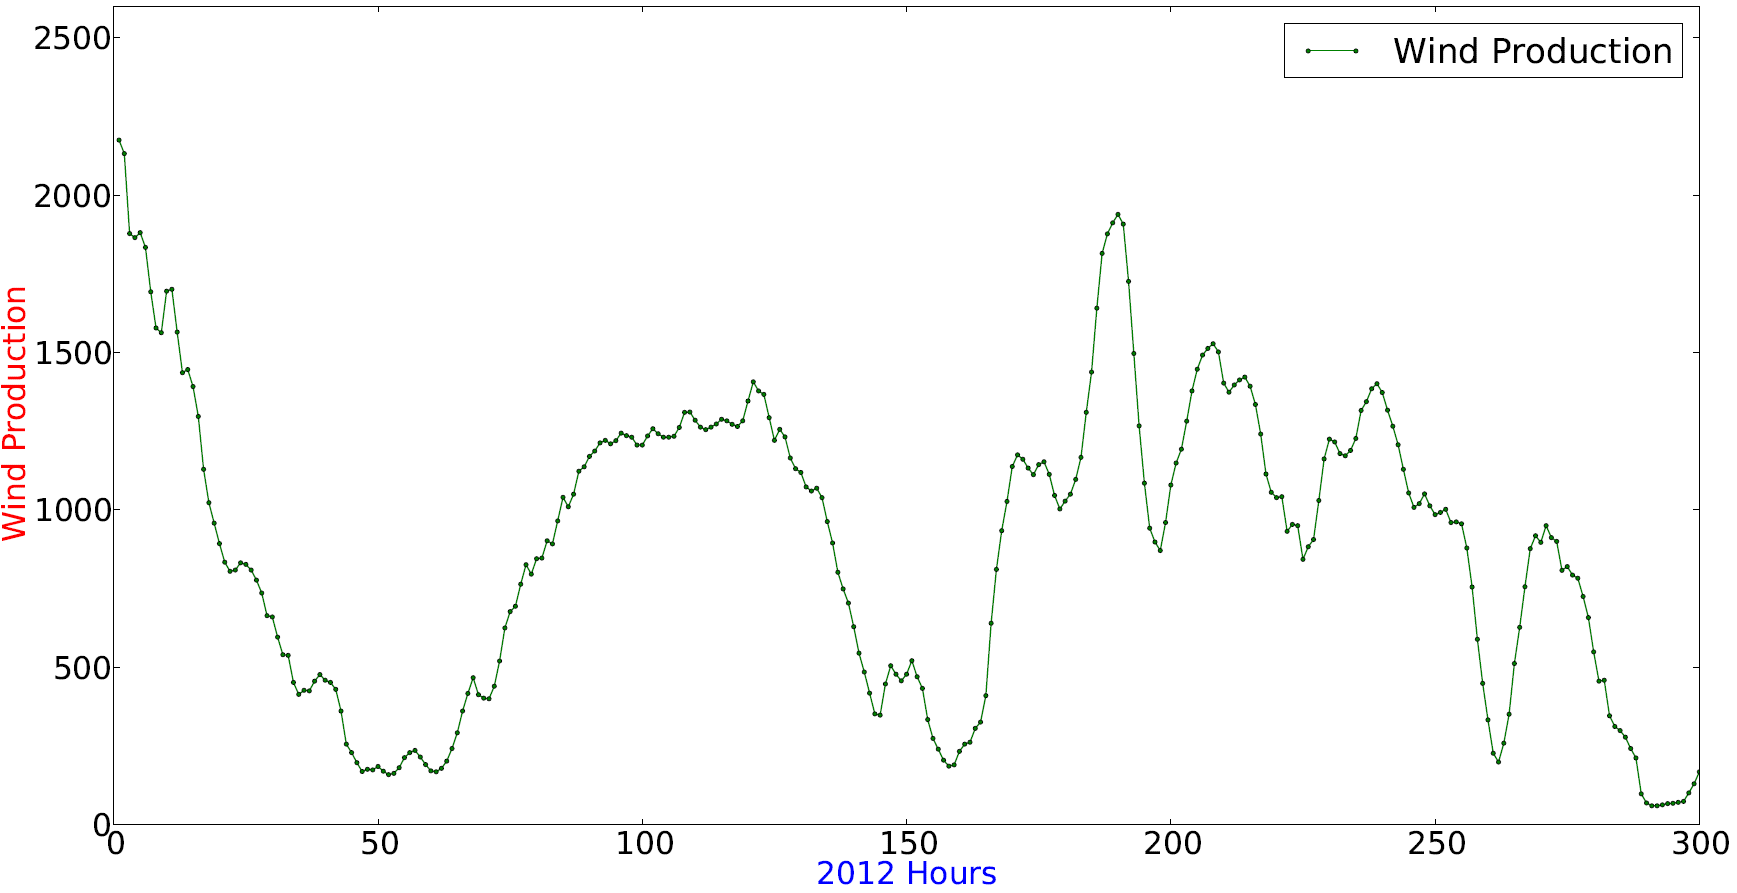
\includegraphics[width=0.99\linewidth,natwidth=898,natheight=587]{billeder/productionTendency400Hours.png}
\caption{Wind production development for 400 hours in 2011}
\label{fig:windHourDevelopment400Hours}
\end{figure}

\begin{figure}[H]
\centering
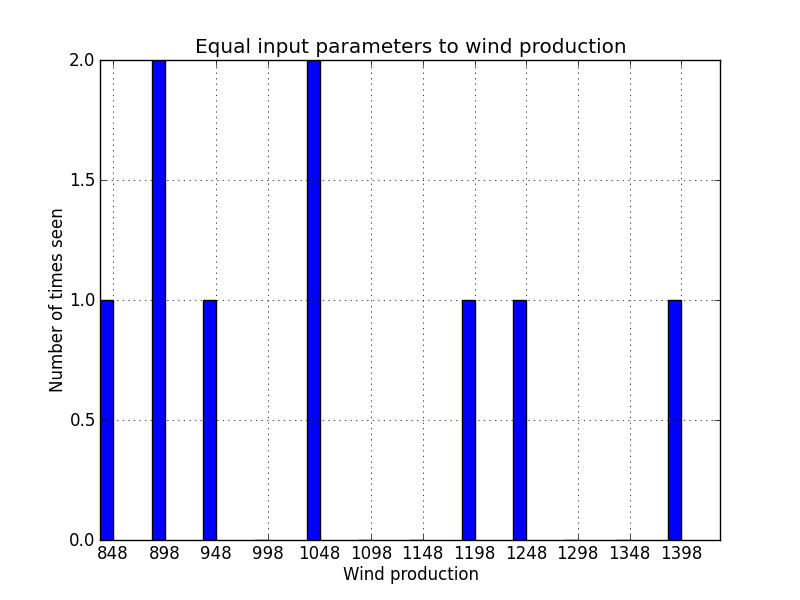
\includegraphics[width=0.99\linewidth,natwidth=898,natheight=587]{billeder/Equal_wind.png}
\caption{Same input parameter to wind production output distribution}
\label{fig:inputParameterDistribution}
\end{figure}

\begin{table}[H]
\centering  % used for centering table
\begin{tabular}{c c c c} % centered columns (3 columns)
 & \#1 Windspeed & \#2 Temperature (Celsius) & \#3 Demand \\ [0.5ex] % inserts table 
%heading
\hline                  % inserts single horizontal line
High margin: & 16.5 & 3.3 & 2359.5  \\
Low margin: & 13.5 & 2.7 & 1930.5 \\ [1ex] % [1ex] adds vertical space
\hline %inserts single line
\end{tabular}
\caption{This is the high and low margins used for the the similar input to output distribution.} % title of Table
\label{table:similarHoursLimitsWindProd} % is used to refer this table in the text
\end{table}

\todo{price irregular price curves}


It is the expectation that the further we get from the start time the less accurate a prediction will be because it uses data from its immediate past to do the prediction. 

\todo{Mention the calculation of the outer percentiles with a neural network for itself}

\todo{Find graph and tell something about the general movements of the wind production. Further more show it together wind wind speed - should see coherence. Use this to locate the irregularities where it does not hold at all}
\todo{write something about that we need to look back}

\todo{In the experiments show a graph of why we add the curve analysis. The network itself tries to do a general fit and because the same input parameters can point to a interval of price/production we need to give the prediction a kind of "snapshop" of the current situation so that it knows which way to go based on the current market situation - we give it more information to base its decision on - if the current input parameters can point to a price between 700-1100 but the price from one hour ago was 900 and the current trend from the last 24 hours is going up then we should probably not guess below 900 - we don't know but since we otherwise would random an answer, the probability of trusting statistics is better. By doing this we can better approach our target to predict}

\subsection{Experimental Results}
This subsection describes the experiments that uncovers the best combination of hidden layers, neurons and epochs as well as the different strategies The ANN will be trained with the hourly parameters of wind speed, temperature, consumption and air density then compared to the actual production of that hour. Furthermore statistical input parameters are included in an attempt to improve accuracy. 

I FOUND RECURRENT LINK IN ARTICLE REF ID

Black art --- experimenting with hidden layers, momentum and learning rate. 


\subsubsection{Experiment One - Data Manipulation}
The first experiment will show the difference in performance due to the manipulation of the time series data set. The three approaches are naive, trimming and matrix. These experiments do not include any statistical features.

\begin{table}[H]
\centering  % used for centering table
\begin{tabular}{c c c c} % centered columns (3 columns)
ANN Type & MAE & MPE & Rank \\ [0.5ex] % inserts table 
%heading
\hline                  % inserts single horizontal line
ANN Naive & 0 & 0 & 0 \\ % inserting body of the table
ANN Trimming & 0 & 0 & 0 \\
ANN Matrix  & 0 & 0 & 0\\
ANN Matrix and Trimming  & 0 & 0 & 0 \\ 
ANN Statistical features  & 0 & 0 & 0\\ [1ex] % [1ex] adds vertical space
\hline %inserts single line
\end{tabular}
\caption{Table showing the performance of different data manipulation approaches when all run with 1500 epochs.} % title of Table
\label{table:dataManipulationApproaches} % is used to refer this table in the text
\end{table}

The purpose is to locate the 

\todo{do 1-12-24 step ahead to show the "carry-with"-error} 

Taking the most naive approach to prediction by simply including the important normalized input parameters and trying to predict the prices for an entire year. 

\subsubsection{Experiment Two - Prediction Strategies}


\subsubsection{Experiment Three - Performance Optimization}
The impact of different Layers/Neurons/Epochs combinations is huge and the results is shown here.

\begin{table}[H]
\centering  % used for centering table
\begin{tabular}{c c c c c} % centered columns (3 columns)
ANN Type & Epochs & MAE & MPE & Rank \\ [0.5ex] % inserts table 
%heading
\hline                  % inserts single horizontal line
ANN & 500 & 0 & 0 & 0 \\ % inserting body of the table
ANN & 1000 & 0 & 0 & 0 \\
ANN & 2000 & 0 & 0 & 0 \\
ANN & 2500 & 0 & 0 & 0 \\ [1ex] % [1ex] adds vertical space
\hline %inserts single line
\end{tabular}
\caption{Table showing the performance of different data manipulation approaches.} % title of Table
\label{table:performanceOpti} % is used to refer this table in the text
\end{table} 

\subsubsection{Experiment One - The idea}
step-ahead from 1 to 24.

